\title{Graphenisomorphie in quasipolynomieller Zeit\\ Der Algorithmus von L\'{a}szl\'{o} Babai}
\author{Yussuf Kassem
        \and
        Benjamin Deutz
        }
\documentclass{article}
\usepackage[ngerman]{babel}
\usepackage[utf8]{inputenc}
\usepackage[T1]{fontenc}
\usepackage{amsmath}
\usepackage{graphicx}
\usepackage{tikz}
\usetikzlibrary{arrows} 
\tikzset{knoten/.style={circle,fill=black,inner sep=1mm}}
\usepackage[section]{placeins}

\usepackage{graphicx}

\newtheorem{theorem}{Theorem}
\newtheorem{example}{Beispiel}
\newtheorem{lemma}{Lemma}
\newtheorem{proposition}{Proposition}
\newtheorem{scolium}{Scolium}   %% And a not so common one.
\newtheorem{definition}{Definition}
\newenvironment{proof}{{\sc Proof:}}{~\hfill QED}
\newenvironment{AMS}{}{}
\newenvironment{keywords}{}{}



\begin{document}
\newpage
\maketitle
\begin{abstract}
Dieses Dokument ist im Rahmen des Kurses \glqq Panorama der Mathematik - Seminar über Fehler\grqq\ im an der Freien Universität Berlin im Sommersemester 2017 entstanden. Es beinhaltet die Ausarbeitung eines Vortrags vom 10. Juli 2017 zum Thema \glqq Graphenisomorphie in quasipolynomieller Zeit\grqq. Dabei wird insbesondere die zeitliche Abfolge der Ereignisse nach der Ankündigung Babais einen quasipolynomiellen Algorithmus gefunden zu haben dargestellt. Das Ziel besteht darin, die Vortragsstruktur und die Inhalte des Themas abzubilden. \end{abstract}

\section{Definitionen}
In diesem Kapitel werden wir die Einstiegsdefinitionen und Notationen festhalten, die für den Vortrag zentral sind.
\begin{definition}
	Ein Graph $G$ ist ein geordnetes Paar $(V, E)$. Dabei ist $V$ eine Menge, deren einzelnen Elemente wir Knoten nennen. $E$ ist die Menge aller Kanten. Jede Kante besteht aus $2$ verschiedenen Knoten.
\end{definition}

\begin{definition}
Gegeben seien zwei Graphen $G = (V,E)$ und $G' = (V',E')$. Dann gilt $G\cong G' \Leftrightarrow \exists \varphi:V\rightarrow V'$ ist eine bijektive Abbildung, für die gilt: $\{v,w\}\in E \Leftrightarrow \{\varphi(v),\varphi(w)\}\in E'$. Wir sagen dann, dass $G$ und $G'$ isomorph zueinander sind. Wir nennen $\varphi$ einen Isomorphismus.
\end{definition}

Diese Definitionen werden im Folgenden an zwei Beispielen anschaulich gemacht. Dazu schauen wir uns zuerst die beiden Graphen in Abbildung \ref{fig:isomorph} an. Durch die Angabe einer Abbildung $\varphi$ kann man erkennen, dass es sich um zwei isomorphe Graphen handelt. Die Abbildung $\varphi$ ist im Folgenden angegeben.

$$\varphi =
    \begin{cases}
    \varphi(a) = 1, \varphi(b) = 6,
    \varphi(c) = 8, \varphi(d) = 3\\
    \varphi(g) = 5, \varphi(h) = 2,
    \varphi(i) = 4, \varphi(j) = 7\\
    \end{cases}  
$$

\begin{figure}
\centering
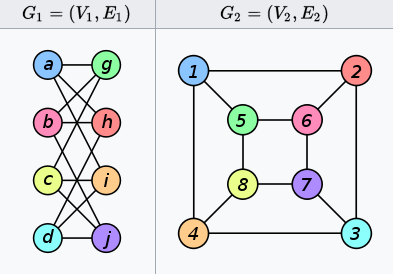
\includegraphics[scale=0.8]{isomorph.png}
\caption{Zwei isomorphe Graphen}\label{fig:isomorph}
\end{figure}


Ein weiteres Beispiel zeigt, dass zwei Graphen, obwohl sie sich auf den ersten Blick vielleicht recht ähnlich sehen, nicht unbedingt isomorph sein müssen. In Abbildung \ref{fig:nisomorph} sehen wir ebenfalls zwei Graphen. Beide haben $5$ Knoten und $6$ Kanten. Um nun argumentieren zu können, warum diese beiden Graphen nicht isomorph sind, brauchen wir eine neue Definition.

\begin{definition}
Gegeben sei ein Graph $G = (V,E)$. Sei $v\in V$ ein beliebiger Knoten. Wir definieren $$d_G(v) := \sum_{e\in E, v\in e} 1.$$
Wir nennen $d_G(v)$ den Grad von $v$. Anders ausgedrückt ist der Grad also die Anzahl aller Kanten, die $v$ mit anderen Knoten verbinden.
\end{definition}

Es ist offensichtlich, dass bei einer isomorphen Abbildung Knoten mit Grad $x$ auf Knoten mit Grad $x$ abgebildet werden müssen.
Wenn wir die Grade aller Knoten in den beiden Graphen betrachten, bemerken wir, dass beide Graphen $3$ Knoten mit Grad $2$ und $2$ Knoten mit Grad $3$ besitzen. Im linken Graphen sind die beiden Knoten mit Grad $3$, nämlich c und d, miteinander verbunden. Im rechten Graphen allerdings sind die beiden Knoten mit Grad $3$ nicht verbunden. Dieses Argument reicht aus, um zu zeigen, dass die beiden Graphen nicht isomorph sein können. 

\begin{figure}
\centering
\begin{tikzpicture}[>=stealth]
    \path node [knoten, label=below:a] (1) at (0,0) {}
          	node [knoten, label=below:b] (2) at (3,0)  {}
          	node [knoten, label=right:c] (3) at (3,3)  {}
          	node [knoten, label=left:d] (4) at (0,3)  {}
          	node [knoten, label=above:e] (5) at (1.5,5)  {}
          	
	     (1) edge (2)
	     (2) edge (3)
	     (1) edge (4) 
	     (3) edge (4)
	     (3) edge (5)
	     (4) edge (5);
	     
	     \path node [knoten, label=below:1] (6) at (7,0) {}
	      node [knoten, label=below:2] (7) at (10,0) {}
	      node [knoten, label=right:3] (8) at (10,3) {}
	      node [knoten, label=left:4] (9) at (7,3) {}
	      node [knoten, label=above:5] (10) at (8.5,5) {}
          		
	     (6) edge (8)
	     (6) edge (9)
	     (9) edge (10)
	     (8) edge (10)
	     (9) edge (7)
	     (7) edge (8)
	     
	     ;
  \end{tikzpicture}
  \caption{Zwei nicht isomorphe Graphen}\label{fig:nisomorph}
  \end{figure}



\section{L\'{a}szl\'{o} Babai}
L\'{a}szl\'{o} Babai ist ein 

\section{Graphenisomorphie - Historie}
In diesem Teil möchten wir einen kleinen historischen Überblick über Ergebnisse im Bereich der Graphenisomorphie geben. Dies schließt die neuesten Erkenntnisse Babais mit ein.

Im September 2015


\begin{thebibliography}{9}
     \bibitem{MyFavorite}
         {\sc Lamport, L.,}
         ``\LaTeX - A Document Preparation System'',
         Addison-Wesley, 1998.

    \bibitem{BobsPaper}
         {\sc Fillioque R.} and {\sc Heliotrope, B.,}
         {\em Why Fermat's last theorem is really a lemma,}
         American Mathematical Weekly,
         Vol. 7, No. 1, pp 115-116, 1998.

\end{thebibliography}



\section*{About the author:}
   We would like a short biographical sketch,
   beyond just your affiliation to be placed
   after the bibliography.
   And below that, your full address.



\subsection*{Primus Scriber}
   College of the Enlightenment,
   Philadelphia, Pennsylvania, 42345-6543$\pm\epsilon$.
   pscriber@cenet.edu

\subsection*{Theco Author}~
   Department of Statistics,
   The Virtual University,
   New York, NY 13291-5555.
   also@aol.com

\end{document}
